\documentclass[b5,twocolumn,11pt]{jarticle}
\usepackage{comment}
\usepackage{amsmath}
\usepackage{graphicx}
\begin{document}

\section{はじめに}
磁性流体とはその名前のとおり, 磁石にくっ付くような性質を持ちながらも容易に(もしくは自発的に)形を変えられる流体の総称である. この性質が磁性流体の最大の特徴と言ってもよく, また工学的にもこの性質を活用したものが多い. 本記事はその磁性流体について, 様々な特性と応用を紹介したものである. 本記事によって皆さんの中に, 磁性流体について興味を持ってくれる方がすこしでも出れば幸いである. また本記事は文献\cite{No7_磁性流体}をもとに, 筆者の磁気混合流体を用いた研磨加工に関する1年間の研究生活を振り返りながら書いたものであるが, 筆者の勉強不足によって誤りや不適切な表現などをを含みうることをはじめに明記しておきたい. 不適切な表現などを発見された方は, ぜひ御一報いただきたい. 

\section{磁性流体とは}
磁性流体( magnetic fluid, ferrofluid, MAGIC fluid )とは, 1960年代から70年代にかけて宇宙技術開発の中で研究がはじまったもので, NASAのSteve Papellにより始めて考案された\cite{No7_SP}. 当初は正常な量の液体燃料をロケットエンジンに供給するための1つのアイディアであったとされ, 燃料に磁性を持たせることができれば無重力下でも磁力により連続的に燃料をエンジンに供給できるのではないかと考えられた. 実際にこのアイディアが実現された様子はないが, 磁性を持った流体というのは非常に汎用性が高く, 応用上の興味も大きい. そのため後にさまざまな改良や工学的な応用が提案され, 今にいたるまで活発に研究が進められている分野となっている. \par
磁性をもつ流体が作りたいというのならばそれに特別な工夫は必要なく, 磁性体粒子を適切な溶媒に混ぜ合わせればよい. 流体というよりもむしろペースト状ではあるが, たとえば磁気回路のコアとして磁性体微粒子を懸濁した磁性材料などが, すでに実用化されている. 問題になるのは, 流体が磁性をもつが一様に磁性体粒子が溶けており沈殿などを起こさないという分散性が必要になった時である. この性質を実現するのは簡単ではないが, この特徴によって特に幅広い応用を考えることができ, 一般的な磁性流体はこの性質を持っている. \par
ここで強調しておきたいことは, 磁性流体は自然に発見されたものではなく, 人工的に機能性を持つように”開発された”流体ということである. この流体は応用的な側面がまず研究され, そのあとに物理的な特性が調べられたという特徴がある. 

  \subsection{作成方法}
まず磁性を流体に持たせるために, 水や石油系の溶媒に磁性体粒子を溶かし込む. 磁気能力の向上のためには飽和磁化の大きな磁性体粒子を用いた方が磁化特性は向上する. \par
しかしながら飽和磁化が比較的大きな純金属の単体を微粒子として用いる場合には空気中での安定性が悪く, $Co$や$Fe$などでは発火の恐れもある. ここで, よく用いられるのはスピネルフェライトというスピノル配位型結晶構造をもつ磁性酸化物であり, その化学式は$AFe_2O_2$で表される\cite{No7_磁気工学の基礎}($A$は$Mn,Co,Ni,Cu,Zn$等). 特にこの中でもっとも飽和磁化が大きなマグネタイトが応用の観点から一般的によく用いられる. \par
また磁性流体に用いる磁性微粒子の大きさは$10nm$($100\AA$)が適当であると考えられている.* これよりも大きすぎると液体中での分散性が悪くなり, これよりも小さいと磁気能力が低下する. この大きさの粒子は原子1つあたりの粒子径の典型的なオーダーである$0.1nm(1\AA)$と大きく変わらないため, 磁性体粒子の酸化膜などの影響が如実に現れやすい. このことからも反応性が高い純金属などは磁性流体にはむいていないことが分かる. また$100nm$は典型的なウイルスの大きさの程度であり$1000nm$(1$\mu m$)が細菌の大きさであることを考えると, この小ささと作成の難しさが直感的に分かると思う. \par
上で述べたような磁性体微粒子の作成にはさまざまな方法がある. NASAによって開発された粉砕法は, 機械的な粉砕により$\mu m$オーダーの磁性体微粒子から数週間かけて$nm$オーダーまで粒子径を落とし込む方法である. そのあと磁性体粒子の粒径を整えるためにさらにデカンテーション(静置)と遠心分離を繰り返す必要がある. 東北大学の研究チームにより開発された共沈法は, 科学的な磁性体粒子の析出を行った後に沈殿とろ過を行い溶媒に希釈するというもので, 工業的な生産が可能である. この他にも溶接の際に飛散した溶鉄を回収する方法があり, これは粒子の形状がきわめて球にちかいと言う特徴があるそうだ. \par
また磁性流体の作成の際に注意すべきこととして, 磁性体粒子をいかにして安定分散させるかというものがある. ここではよく用いられている界面活性剤による分散化手法について述べる. 界面活性剤は親水基と疎水基を持ち, 疎水基が図\ref{fig:sd}に示したように磁性体粒子の表面に吸着する. この界面活性剤は磁性体粒子間の距離を一定以上に保つための重要な役割を果たす. 磁性流体中では距離が小さくなると磁性体粒子間の引力は大きくなるため, なにか間にはさまないと互いに凝集してしまう. なぜなら磁性体粒子に働く相互引力ののうち, 磁気双極子相互作用が$1/r^3$のオーダーで与えられ, ファンデルワールス力が$1/r^7$程度のオーダーで与えられるからである. それをふせぐため界面活性剤を磁性体粒子にくっつけ, 分子鎖同士を反発させて弾性力として働かせることで, 粒子の凝集をふせぎ分散性を向上させることができる. 実際には少なくともオレイン酸程度の長さの分子鎖をもつ界面活性剤が望ましいようである. \par
*$10nm$程度の磁性体微粒子を用いた磁性流体にさらに特性の向上のために1$\mu m$オーダーの鉄粉を添加し, 磁気能力を向上させたものとして磁気粘性流体がある. この流体中で鉄粉は安定に分散しておらず, 数時間で沈殿する. (磁気混合流体を用いた研磨加工の項を参照のこと)

\begin{figure}
\begin{center}
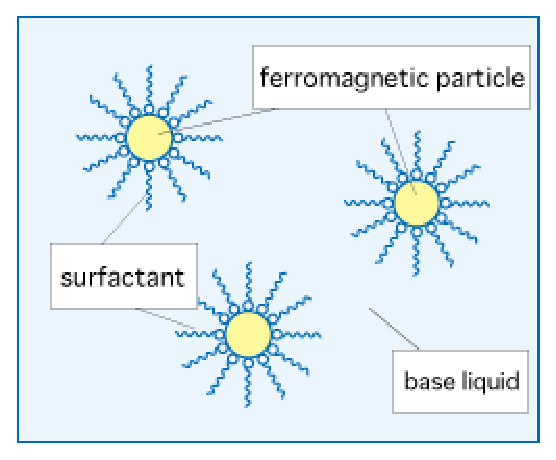
\includegraphics[width=70mm]{No17_sd.eps}
\end{center}
\caption{分散性の模式図}
\label{fig:sd}
\end{figure}

\section{磁性流体の物理的な特性}
繰り返しになるが磁性流体とは磁性を持った流体の総称で, 磁性体粒子の材質や溶媒, 混合比率, 応用のための添加物などに自由度があるためその種類は多岐にわたる. ここではその一般的な性質について説明を行う. \par
なお定性的に現象を扱うため本章でしめした式の導出の際, いくつかの仮定と近似を行っているが詳細は省略した. 詳しくは文献\cite{No7_磁性流体}\cite{No7_MF}などを参照されたい. 

  \subsection{磁性}
まず反磁場について述べておこう. 反磁場とは, 磁場のもとで磁性体が磁化するときに端面にできる仮想的な磁極が, 内部のもともとの磁場を打ち消すようにできる磁場のことである. この効果が磁性流体では比較的に重要となり, 実効的な透磁率は大きくなりにくい. これは磁性流体でできる仮想的な磁極が流体界面ではなく粒子の端面でできるためである. この効果に対する評価は, 例えば松野ら\cite{No7_反磁場}によって行われている. なお反磁場とは反磁性とはまったく異なる概念であることを注意しておく. \par
また磁性流体に含まれる磁性微粒子は一般に, 一粒子全体の回転による回転ブラウン運動や粒子内部の磁化の回転を意味するネール回転により, 磁化が簡単に変化しうる. これはおもに粒子の粒径が小さいことによるもので, 強磁性体粒子が常磁性体のような特性を持つことから超常磁性( superparamagnetism )と呼ばれる. \par
ここで注意しておきたいのは, 薄膜やバルク型試料と異なり磁性流体の磁化特性を計測するのはけっして簡単な作業ではないということだ. 磁性流体の場合, 流動性を持つので磁性体粒子が流体中で移動するが, そうなると体積あたりの磁化は試料を密封する容器の形状によって異なることがある. これは厄介な性質だ. しかしながら複素透磁率や飽和磁化などを知りたいと言う要請は大きく, 例えば磁気混合流体については\cite{No7_MCF磁気特性}に詳しく調べられている. 

  \subsection{界面現象}
磁性流体はその特性から, 黒色で非透明であって観察が難しい. そこで液面での界面現象をみることが重要になってくる. もちろん界面現象はさまざまな状態が考えられるが, 図\ref{fig:MF}のように表面にスパイクができたものは審美的な観点からも美しく有名であろう. 一瞬でよく目を凝らさないと分からないが, 2014年のレクサス(Rexus RC 300/350h)の商業的なCMに使われたほどでもある. \par
さて磁性流体の平衡状態では界面の圧力は大気圧に等しく, 一般化されたベルヌーイの式によって式\ref{eq:No7_Bernoulli}のように表される. $\vec{M}_{\perp}$は磁化ベクトルの界面に垂直な成分であり, $\phi = \int_{H}^{H_0} M dH $は磁気ポテンシャルである. 

    \begin{equation}
      z = \frac{\phi}{\rho g} + \frac{(\vec{M}_{\perp})^2}{2\mu_0} + C \label{eq:No7_Bernoulli}
    \end{equation}

\begin{figure}
\begin{center}
\includegraphics[width=70mm]{No17_MF.eps}\\
\end{center}
\caption{磁性流体の界面現象}
\label{fig:MF}
\end{figure}


この式から図に示したようなスパイクのおおまかな特性が説明できるが, 磁場を大きくしてゆきスパイクができはじめる際の臨界現象, またどのように規則的な突起が形成されるかについては説明できない. 理解のためには本質的にナビエ・ストークス方程式を解く必要があるため, 解析は非常にむずかしい. 

  \subsection{磁気浮揚効果}	
磁気浮揚効果とは磁性流体中の非磁性体粒子がまわりとの圧力差から力を受け, 移動する現象であり磁気浮力現象とも呼ばれる. \par
まず浮力とは一般に, 圧力分布に偏りがあるような流体中で物体が感じる圧力差が力となって現れるものである. 非磁性体粒子に作用する圧力差を流体力学と磁気の知識を用いて書き下すと, 式\ref{buo}が近似的に導かれる. 磁性体の磁場中でのポテンシャルエネルギー $U=- \vec{M} \cdot \vec{H}$と$F=-\nabla U$を用いて磁化Mが一定であるとしたとき分かりやすい. 

    \begin{align}
      F & = \int_S \vec{M} \cdot \vec{H} d\vec{S} \nonumber \\
        & = \int_V \vec{M} \cdot \nabla \vec{H} dV \label{buo}
    \end{align}

さらに直感的には, 我々が感じるような水の中での浮力との対比を行うと良い. 水の中で我々が感じるような浮力はアルキメデスの原理によって説明されるが, この原理は物体が押しのけた分の水に働く重力と等しいだけの力が, 物体に浮力として重力と逆方向にはたらくというものである. これは磁性流体においても同様で, 非磁性体粒子が押しのけた分の磁性流体にはたらく磁力が, 非磁性体粒子に逆方向の浮力としてはたらく. 

\section{磁気機能性流体の工学的応用}
磁気混合流体は磁性に感応して制御の行える数少ない流体ということもあって, その応用は多岐に渡っており工学的応用から医学的な観点まで幅広い. ここでは磁気混合流体を用いた研磨加工に焦点を絞って述べる. 上記のような応用に興味のある方は文献\cite{No7_磁性流体}などを参照されたい. なお応用に関して提案されているものの一部を下に列挙する. \\
Keyword:加速度センサ, 傾斜計, 圧力計, 光モジュレータ, スピーカ, アクチュエータ, 比重差選別装置, 粘性ダンパー, 軸受(シール), 磁性紙, ドラッグデリバリー, 温熱療法(がん細胞など)\par

     \subsection{磁気混合流体}
現在, 精密鏡面加工などの研磨加工は高い精度と小さな表面荒さの実現のため, 人の手で行われることが多いがこれには費用がかかる. また人の手でもロボットアームでも細い円管内面などは研磨を行うことが難しい. 磁性流体を用いた研磨加工が実現されると現在の難点が解消し, 機械的な自動化が可能になり, 砥粒の支持圧が低いという特徴から表面変質が小さくなる. 実験的に磁性体を研磨加工することは難しいことが分かっているが, 非磁性体に関しては既に実用化されており, 商業ベースに乗っているものもある. 例として西田らによって報告されているものを挙げておく\cite{No7_研磨}.\par
しかしながら磁気混合流体を用いた研磨加工に磁性流体そのものをもちいることはできない. 一般に研磨(ポリシング)にはひっかき硬度が高い砥粒が必要であるが, 磁性流体に含まれる磁性体粒子ではその硬度が十分でないからである. この際, 磁性流体に粒径の異なる鉄粉($1\mu m$程度)を加え磁気能力を高めた磁気粘性流体(MRF: Magnetorheological fluid)を用いて, さらに$\alpha$-セルロースなどの有機物粉末を添加し剪断応力(粘性)を向上させるなどの工夫が行われる. MRFは磁場のもとで異なる粒径の磁性体粒子が鎖状の磁気クラスタと呼ばれる構造を持ち見かけの上での粘性が上昇する. この磁気クラスタは磁性流体に含まれる磁性体微粒子のみでもできるが, MRFでは特に弾力性にとむ長いクラスタができることが分かっている. しかしこの流体は分散性が悪く, 懸濁処理が必要である. 

\begin{thebibliography}{99}

  \bibitem{No7_磁性流体}
山口博司 (2011). 磁性流体, 森北出版.

  \bibitem{No7_SP}
US Patent \# 3215572 filed Oct 9, 1963

  \bibitem{No7_磁気工学の基礎}
太田恵造 (1973). 磁性流体, 森北出版.

  \bibitem{No7_MF}
Ronalds E. Rosensweig (1987). Magnetic Fluids, Annual Review of Fluid Mechanics, Vol 19, pp.437-461.

  \bibitem{No7_反磁場}
Yoshiyuki Matsuno, Hiroharu Fujise, Kazuya Tomosawa, Yasutake Hirota(1996-1997). Demagnetizing Factor of Magnetic Fluid, Transactions of the Japan Society of Mechanical Engineers, Series B, vol 62, No 599.

  \bibitem{No7_MCF磁気特性}
Kunio Shimada, Hideo Oka (2005). Magnetic characteristic of magnetic compound fluid (MCF) under DC and AC magnetic fields, Journal of Magnetism and Magnetic Materials vol 290-291 pp.805-807.

  \bibitem{No7_研磨}
 Hitoshi Nishida, Kunio Shimada, Ichro Yoshino (2012). Study of Micro Processing for Inner Tube Walls Utilizing Magnetic Compound Fluid, Journal of Japanese Society for Experimental mechanics, vol 12, No 4, pp.361-368. 

\end{thebibliography}

\end{document}
